% !TEX encoding = UTF-8 Unicode
\documentclass[11pt, a4paper]{article}

\usepackage{todonotes}

% Setup of packages used
\usepackage[onehalfspacing]{setspace}		% One half spacing
\newlength{\stockheight}					% To prevent hyperref warning
\setlength{\stockheight}{\paperheight}		% define \stockheigh
\usepackage{hyperref}					% Hyperlinks on pdf (Should be called before Geometry)
\usepackage[a4paper, 					% Page Layout
                     %showframe,				% This shows the frame
                     includehead,
                     footskip=7mm, headsep=6mm, headheight=4.8mm,
                     marginparsep=2mm, marginparwidth=22mm,
                     top=25mm, bottom=25mm, inner=30mm, outer=25mm]{geometry}
\usepackage{sansmathfonts}				% Sans Serif equations
\usepackage[T1]{fontenc}					% Output font encoding for internationa

\usepackage[utf8]{inputenc}			% Encoding of files: utf8
\renewcommand*\familydefault{\sfdefault} 	% Sans Serif as default font
\usepackage{titlesec}					% Redefine chapter and chapter* titles
\titleformat{\chapter}[display]{\huge \bfseries}{\vspace{-0.5cm}\hfill \chaptertitlename\ \thechapter}{0pt}{\hfill}[{\titlerule[1.2pt]}]
\titleformat{name=\chapter,numberless}[display]{\huge \bfseries}{\vspace{-0.5cm}}{0pt}{\hfill}[{\titlerule[1.2pt]}]

% This is used to include the page number on footer within the same margins
%\titleformat{\chapter}[display]{\huge \bfseries}{\vspace{-0.5cm}\hfill \chaptertitlename\ \thechapter}{0pt}{\hfill}[{\titlerule[1.2pt] \enlargethispage{-0.75\baselineskip}}]
%\titleformat{name=\chapter,numberless}[display]{\huge \bfseries}{\vspace{-0.5cm}}{0pt}{\hfill}[{\titlerule[1.2pt] \enlargethispage{-0.75\baselineskip}}]


\usepackage{fancyhdr}					% Package to redefine headers
\fancyhf{}								% No header nor footer
\fancyhead[L]{\thepage}				% Left even and right odd Page Number
\pagestyle{fancy}

\fancypagestyle{plain}{					% To change the footer on chapter and chapter*
	\fancyhf{}							% No header nor footer
%	\fancyfoot[C]{\vspace{-11mm}\thepage}	% Footer with number displaced
	\renewcommand{\headrulewidth}{0pt}	% No line on header
	\renewcommand{\footrulewidth}{0pt}		% No line on footer
}

\RequirePackage{caption} 				% Caption customization
\captionsetup{justification=centerlast,font=small,labelfont=sc,margin=1cm}

\hypersetup{
    colorlinks=true,
    linkcolor=blue,
    filecolor=magenta,      
    urlcolor=blue,
    citecolor=blue,    
}

% Setup the language and its properties (choose only one)
\usepackage[spanish, es-tabla, es-nodecimaldot]{babel}
\addto\captionsspanish{\renewcommand{\contentsname}{Contenido}}
%\usepackage[english]{babel}
%\addto\captionsenglish{\renewcommand{\contentsname}{Contents}}


%\graphicspath{ {figs/} }					% Use this if custom figures folder is needed
\setlength{\parindent}{0pt}
\usepackage{amssymb,amsmath}
\usepackage[square, numbers]{natbib}		% Bibliography
\usepackage{tikz}						% Required for title page
\usetikzlibrary{babel}						% Required to make TikZ works with babel
\usepackage[section]{placeins}				% To flush floats before new section
\usepackage{longtable}					% Used by List of Symbols and friends
\usepackage{array}						% Needed by longtable package
\usepackage{graphicx}

%para el color del texto
\usepackage{color}

%para poder poner H en imagenes
\usepackage{float}

%para poder importar excel
\usepackage{csvsimple}
\usepackage{booktabs}

%Para dibujar circuitos
\usepackage{circuitikz}


% Macros provided
\def\fecha{\ifcase\month\or
  Enero\or Febrero\or Marzo\or Abril\or Mayo\or Junio\or
  Julio\or Agosto\or Septiembre\or Octubre\or Noviembre\or Diciembre\fi \space\number\year
}
\newcommand*{\subtitle}[1]{\gdef\@subtitle{#1}}
\newcommand*{\group}[1]{\gdef\@group{#1}}
\newcommand*{\profesor}[1]{\gdef\@profesor{#1}}

\begin{document}
% !TEX encoding = UTF-8 Unicode
% !TEX root = ../thesis.tex
\title{TRABAJO PR\'ACTICO N\textsuperscript{\underline{o}}2: Ej 8}
\group{Grupo II}
\author{ \newline Pablo Mart\'in  \textsc{Scheinfeld} (59065), \newline
Santiago Agustín \textsc{Arribere} (59169), \newline
Matías Santiago \textsc{Francois} (59828), \newline
Rafael Nicolás \textsc{Trozzo} (59434), \newline
Gonzalo Joaquín \textsc{Davidov} (59117)}

\profesor{\newline Kevin \textsc{Dewald}, \newline
Pablo Enrique  \textsc{Wundes}, \newline
Miguel \textsc{Aguirre}}
\date{\fecha}
\begin{titlepage}
	\onehalfspacing
	\enlargethispage{0.65\baselineskip}
	\begin{tikzpicture}[remember picture, overlay]
		\coordinate (top_right) at 
		    ([xshift=-2.5cm, yshift=-2.5cm]current page.north east);
		\coordinate (top_left) at 
		    ([xshift=2.3cm, yshift=-1.8cm]current page.north west);
		\coordinate (bottom_right) at 
		    ([xshift=-1.8cm, yshift=1.8cm]current page.south east);
		\node[inner sep=0, anchor=north east] at (top_right) {\href{http://www.itba.edu.ar}{
\includegraphics[height=19mm, trim={180 200 200 200}, clip]{figs/logo_itba.png}}};
		\draw[double, line width = 0.5pt] (top_left) rectangle (bottom_right);
	\end{tikzpicture}
	\par
%	\begin{large}
		\vspace{-1cm}
		\noindent \textbf{22.13 - ELECTR\'ONICA III}\par
		\vspace{4cm}
		\begin{center}
			{\Huge \textbf{\@title}\par}
			\vspace{1cm}
			{\huge \textbf{\@subtitle}\par}
			\vspace{1cm}
			{\Large \textbf{\@group}\par}
		\end{center}
		\vfill
		\noindent \textbf{AUTORES:} \@author \par
		\vspace{1cm}
		\noindent \textbf{PROFESORES:} \@profesor \par
		\vspace{1cm}
		\begin{center}
			\textbf{CIUDAD AUTÓNOMA DE BUENOS AIRES}\\
			\textbf{\@date}\par
		\end{center}
%	\end{large}
\end{titlepage}
\setcounter{tocdepth}{2}
\tableofcontents
\newpage
%
\section{Introducci\'on}
El objetivo del presente trabajo es leer la posici\'on de un \textit{joystick} y mostrarla en un \textit{display} representada por numero entre 0 y 99, con una tasa de refresco de entre 1 y 20 veces por segundo. El \textit{joystick} est\'a compuesto por un potenci\'ometro en cada eje y es alimentado con 5V por lo tanto a la salida se tendr\'an tensiones entre 0V y 5V. Se busca mostrar esa se\~nal en un \textit{display} 7 segmentos de forma que si la tensi\'on es m\'inima, se muestre un 0, con el aumento de la tensi\'on crezca linealmente el n\'umero y si se tiene tensi\'on m\'axima se muestre un 99.
\newpage

\section{Modularizaci\'on del circuito}
%
A continuaci\'on se explican los dos m\'odulos en los que separ\'o el trabajo, uno encargado de la conversi\'on de anal\'ogico a digital y el otro encargado de mostrar el n\'umero.
\subsection{Conversi\'on de anal\'ogico a digital}
%
Como la señal de entrada es anal\'ogica, y se la quiere representar de manera digital, se requiere realizar una conversi\'on de la señal anal\'ogica a valores digitales. Para su realizaci\'on, se genera una se\~nal triangular con \textit{duty-cycle} del 50\%, de la cu\'al se utiliza \'unicamente la parte creciente. Se tiene al mismo tiempo un contador contando a una frecuencia 200 veces mayor que la de la tri\'angular para lograr que cuente de 0 a 99 durante la subida. Mientras la triangular baja, el contador se reinicia, para volver a contar al comenzar nuevamente la subida de la señal. \\
En cuanto a la frecuencia, como la tasa de refresco ser\'a de hasta 20$Hz$, la triangular se hace de 50$Hz$ para asegurarse que en cada refresco haya un nuevo valor de la posici\'on. Por lo tanto, la frecuencia del \textit{clock} del contador debe ser de 10$kHz$.\\
La tensi\'on de la triangular va de 0 a 5V y se la compara con la del \textit{joystick}, de modo que cuando la triangular supera al joystick, se deshabilita el contador, y queda guardado un n\'umero que representa la posici\'on del \textit{joystick}. Si la tensi\'on de entrada fuera de 0V, la triangular siempre ser\'ia mayor, y el valor de la cuenta ser\'ia siempre 0. Por otro lado, si la tensi\'on de entrada fuera 5V, la triangular nunca la superar\'ia y la cuenta ser\'ia 99. \\
Como el contador solo tiene valores v\'alidos de la posici\'on del \textit{joystick} desde el momento en que la triangular supera la tensi\'on de entrada, hasta que la triangular comienza a bajar, se debe guardar en ese intervalo de tiempo el valor para luego mostrarlo en el display. Para almacenar el valor se usa un registro formado por Flip-Flops D, es decir, un registro sincr\'onico. Para ello, con un comparador se compara la tensi\'on de entrada con la de la triangular, de modo que cuando la segunda supera a la primera, la salida del comparador pasa de 5V a 0V, y se utiliza dicho flanco para almacenar el valor, conectando la salida del comparador negada al \textit{clock} del registro. Adem\'as, la salida del comparador se conecta al \textit{enable} del contador.\\
En la Figura \ref{fig:diag_temp_ADC} se muestra un diagrama temporal de la situaci\'on descripta. Se puede apreciar que el contador va cambiando de valor durante la subida de la triangular, que en este caso se representa con 'clkTriang' en estado alto, mientras que el registro siempre tiene un valor v\'alido de la posici\'on del \textit{joystick}.
%
\begin{figure}[H]
	\centering
	\resizebox{0.9\linewidth}{!}{
			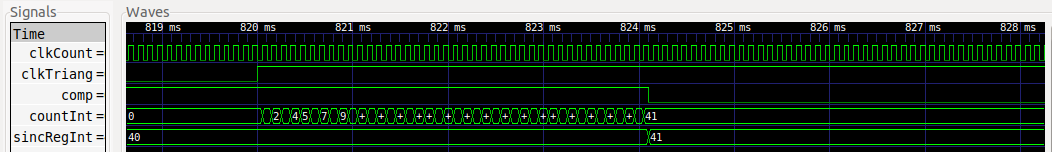
\includegraphics{figs/diag_temp_mod1.png}	
	}
	\caption{Diagrama temporal de la conversi\'on de anal\'ogico a digital.}
	\label{fig:diag_temp_ADC}
\end{figure}
%
\subsection{Visualizaci\'on en display 7 segmentos}
\label{sec:mod_visual}
Para mostrar los valores se utiliza un modulo que recibe los valores v\'alidos de la posici\'on del joystick obtenidos por el contador y se encarga de mostrarlos con una tasa de refresco variable entre 1 y 20$Hz$. Para ello se tiene un registro asincr\'onico, un conversor de BCD a 7 segmentos y un clock de frecuencia variable. \\
El registro asicnr\'onico se utiliza ya que, si bien el registro sincr\'onico siempre tiene valores v\'alidos, podr\'ia ocurrir que en el momento en que haya que refrescar el display cambie el valor del registro, lo cual conducir\'ia muy probablemente a errores en la muestra. Para evitar \'este problema, se agrega un registro m\'as, que siempre tiene a la salida el valor que provee el registro sincr\'onico, excepto mientras se refresca el display, intervalo durante el cual no cambia su valor. \'Esto se logra con un registro hecho con Latch D, que tiene su entrada conectada al registro sincr\'onico y su enable conectado al clock de la tasa de refresco. Mientras el clock de la tasa de refresco est\'a en estado bajo, el latch se deshabilita, imposibilitando que cambie su valor.\\
El esquema explicado anteriormente funciona con un \textit{clock} con muy poco tiempo en estado bajo, con lo que no hace falta un \textit{edge detector}, y durante ese corto tiempo se deshabilita el registro asincr\'onico y se habilita la escritura del display, conectando el \textit{clock} al \textit{Latch Enable} del conversor de BCD a 7 segmentos.\\
En la Figura \ref{fig:diag_temp_total} se muestra un diagrama temporal del funcionamiento de todo el circuito con la tasa de refresco fija en 20$Hz$, en un punto en el que un cambio en el registro sincr\'onico por un flanco descendente del comparador cae en el mismo momento que se est\'a actualizando el display ya que 'clkDisp' est\'a en estado bajo. Se puede apreciar que el registro asincr\'onico siempre copia el valor del registro sincr\'onico excepto cuando el clock de la tasa de refresco est\'a en estado bajo, que a su vez es el \'unico intervalo de tiempo durante el cual el display cambia su valor. De no estar el registro asincr\'onico, en \'este caso la salida del display hubiera cambiado de 96 a 97 durante la actualizaci\'on, y si estos cambios no respetaran los tiempos de set-up y de hold del conversor de BCD a 7 segmentos el comportamiento estar\'ia indefinido.
%
\begin{figure}[H]
	\centering
	\resizebox{0.9\linewidth}{!}{
			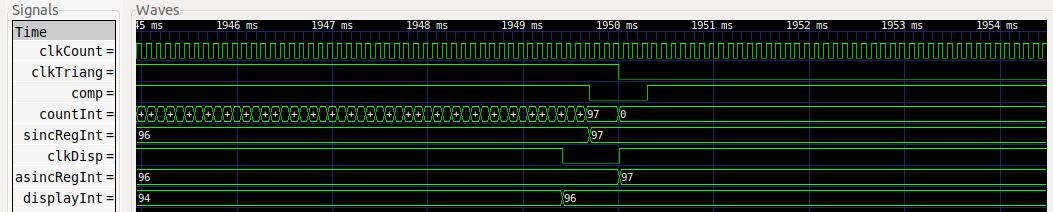
\includegraphics{figs/diag_temp_glitch_evitado.png}	
	}
	\caption{Diagrama temporal de todo el diseño.}
	\label{fig:diag_temp_total}
\end{figure}
%
\newpage
\section{Generaci\'on de señales}
Los m\'odulos ya explicados precisan generar tanto señales de clock como la señal triangular utilizada para comparar con el \textit{joystick}.
A continuaci\'on se explican los circuitos necesarios para generar dichas señales.
\subsection{Señal triangular}
%
\subsubsection{Circuito}
%
Para la generaci\'on de la señal triangular se opt\'o por generar una onda cuadrada con un amplificador operacional utiliz\'andolo con realimentaci\'on positiva y causando su saturaci\'on en $V_{cc}$ y $-V_{cc}$, para luego integrar dicha onda cuadrada y as\'i obtener una triangular, utilizando para ello el circuito de la Figura \ref{fig:gen_triangular}. El circuito de arriba a la izquierda genera la onda cuadrada y el de abajo a la izquierda es el integrador. El circuito de arriba a la derecha ajusta la cuadrada, y el de abajo a la derecha ajusta la triangular.
%
\begin{figure}[H]
	\centering
	\resizebox{0.8\linewidth}{!}{
			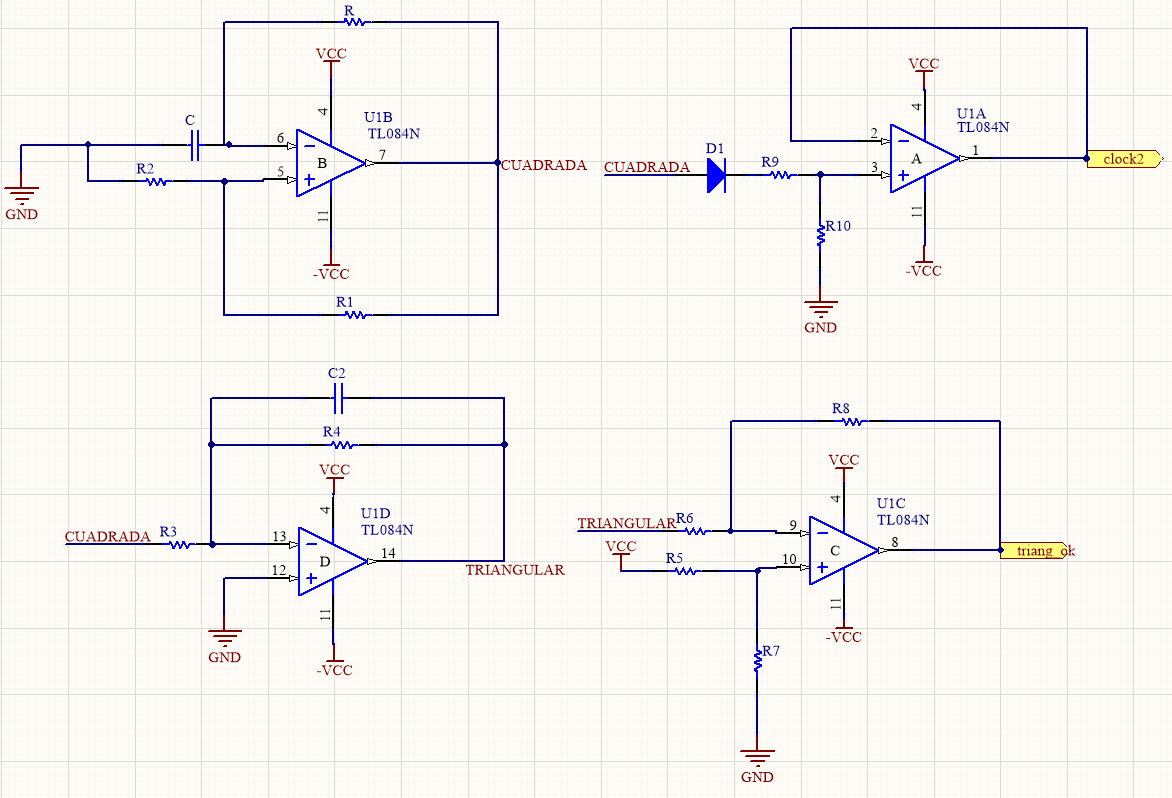
\includegraphics{figs/triang.png}	
	}
	\caption{Generador de onda cuadrada y triangular.}
	\label{fig:gen_triangular}
\end{figure}
\noindent
Para la onda cuadrada, el per\'iodo viene dado por:
\begin{equation}
    T = 2 R C ln \left ( \frac{1 + \beta}{1 - \beta} \right )
\end{equation}
Con $\beta = \frac{R_2}{R_1 + R_2}$. Tomando $R_1$ = $R_2$, se tiene:
\begin{equation}
    T = 2 R C ln(3)
    \label{eq:clk2_freq}
\end{equation}
%
Luego, la cuadrada pasa por el integrador compensado, cuya transferencia viene dada por:
\begin{equation}
    H(s) = \frac{-\frac{R_4}{R_3}}{1 + s C_2 R_4}
\end{equation}
Se observa que la frecuencia de corte, a partir de la cual comienza a integrar, es:
\begin{equation}
    f_c = \frac{1}{2 \pi R_4 C_2}
\end{equation}
Para asegurarse una correcta integraci\'on se busca que: 
\begin{equation*}
    f_c < 10 f
\end{equation*}
Siendo f la frecuencia de la señal a integrar.\\
Por \'ultimo, para ajustar los valores de ambas señales a las necesidades del circuito, se utilizan los circuitos restantes de la figura. Para llevar la cuadrada de 0 a 5V, se agregan un diodo y un divisor resistivo, y se coloca un buffer a la salida para mantener constante dicha tensi\'on. La tensi\'on a la salida del buffer es de:
\begin{equation}
    V_{cuad} = V_{sat} \frac{R_{10}}{R_9 + R_{10}}
\end{equation}
Como la triangular no arranca desde 0V, se coloca el circuito sumador inversor con el cuarto amplificador operacional, para poder sumarle la tensi\'on necesaria para que arranque de 0V. En caso de tambi\'en querer ajustar la tensi\'on pico a pico de la triangular, se puede hacer con las resistencias $R_6$ y $R_8$. La tensi\'on a la salida del sumador inversor se obtiene mediante:
\begin{equation}
    V_o = - \Lambda(t) \cdot \frac{R_{8}}{R_{6}} + V_{cc}\cdot \frac{R_7}{R_5 + R_7} \frac{R_6 + R_8}{R_6} 
\end{equation}
%
\subsubsection{Selecci\'on de valores de componentes}
\noindent
Para la obtenci\'on de la señal cuadrada de 50$Hz$, utilizando la Ecuaci\'on \ref{eq:clk2_freq} se fija el valor del capacitor C=470$nF$ y las resistencias $R_1=R_2=100k\Omega$ para tener corrientes bajas pero sin llegar a $M\Omega$ para no introducir ruido. Con estos valores se obtiene $R=19366\Omega$. Como el valor de \'esta frecuencia debe ser muy preciso, se coloca un preset de 50$k\Omega$ en el lugar de R para ajustarla.\newline
Luego, para el circuito integrador, 
%
\subsection{Señal de clock con NE555}
%
\subsubsection{Circuito}
Para generar dos de las señales de \textit{clock} del circuito se utiliza el circuito de la Figura \ref{fig:clock_555}. 
%
\begin{figure}[H]
	\centering
	\resizebox{0.6\linewidth}{!}{
			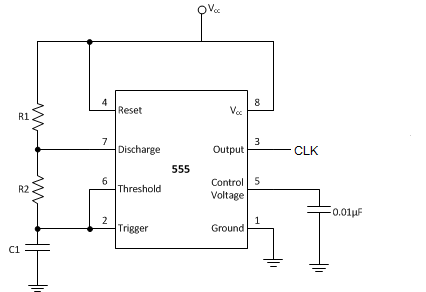
\includegraphics{figs/555_timer.png}	
	}
	\caption{Generador de clock con NE555.}
	\label{fig:clock_555}
\end{figure}
%
Resolviendo la carga y descarga del capacitor C, se tiene que los tiempos en estado alto y en estado bajo vienen dados por:
\begin{align}
    t_H &= ln(2) \cdot C_1 \cdot (R1 + R2) \\
    t_L &= ln(2)\cdot C_1 \cdot R_2     
    \label{eq:555_clk_times}
\end{align}
%
Siendo la señal en estado alto aproximadamente $V_{cc}$, y en estado bajo aproximadamente 0V. Sumando ambos tiempos se obtiene el periodo e invirtiendo se obtiene la frecuencia:
%
\begin{equation}
    f=\frac{1}{ln(2) \cdot C \cdot (R_1 + 2R_2)}
    \label{eq:555_clk_freq}
\end{equation}
\label{sec:clk_variable}
%
Para el caso en el que se necesita una frecuencia variable, se coloca un potenci\'ometro de resistencia $R_{pot}$ en serie a una resistencia $R$ en el lugar de $R_1$. Por lo tanto, se tienen las siguientes ecuaciones para las frecuencias:
\begin{equation}
    \begin{cases}
        f_{min} = \frac{1}{ln(2)C_1(R + R_{pot} + 2 R_2) } \\
        f_{max} = \frac{1}{ln(2)C_1(R + 2 R_2)}
    \end{cases}
\end{equation}
\noindent
Resolviendo para las resistencias que forman $R_1$, y con $\Delta f = f_{max} - f_{min}$, se tiene que:
\begin{equation}
    \begin{cases}
    R = \frac{1}{f_{max}ln(2)C} - 2 R_2 \\
    R_{pot} = \frac{\Delta f}{f_{min} f_{max} ln(2) C}
    \end{cases}
    \label{eq:555_var_clk_R}
\end{equation}
%
\subsubsection{Selecci\'on de valores para el contador}
\noindent
Para el \textit{clock} del contador, se busca una frecuencia de 10$kHz$, que viene dada por la Ecuaci\'on \ref{eq:555_clk_freq}. Se elige un capacitor de 180$nF$ y $R_2$ de 100$\Omega$, con lo que se precisa $R_1$ de 601,5$\Omega$. Dado que la frecuencia de \'este \textit{clock} es determinante para el correcto funcionamiento del circuito, en el lugar de $R_1$ se coloca un \textit{preset} de 1$k\Omega$ para poder ajustarla. 
%
\subsubsection{Selecci\'on de valores para la tasa de refresco}
\noindent
Para el \textit{clock} variable de la tasa de refresco, como se explic\'o en la subsecci\'on \ref{sec:clk_variable}
se coloca en el lugar de $R_1$ una resistencia $R$ en serie con un potenci\'ometro de valor $R_{pot}$.
Se dispone de los valores de potenci\'ometros de la Tabla \ref{tab_pot_comerciales}.

\begin{table}[H]
\center
\begin{tabular}{|c|c|c|c|c|c|c|c|}
\hline
Valor [$\Omega$] & 1 k & 10 k & 100 k & 250 k & 500 k & 50 k & 500 k \\ \hline
\end{tabular}
\caption{Valores disponibles de potenci\'ometros.}
\label{tab_pot_comerciales}
\end{table}

\noindent
Se buscan valores de C entre 1$\mu F$ y 10$\mu F$, porque valores m\'as pequeños exigen valores de $R_{pot}$ del orden de los $M\Omega$ y mayores s\'olo pueden ser alcanzados con capacitores electrol\'iticos de muy mala tolerancia y gran tamaño. Teniendo \'esto en cuenta, con los valores buscados de $f_{min}$ y $f_{max}$, y con los valores comerciales disponibles de C, el valor de $R_{pot}$ m\'as cercano a los disponibles es de 290$k\Omega$, con $C$ = 4,7$\mu F$. Para lograr este valor, se utiliza un potenci\'ometro de 500$k\Omega $ en paralelo con una resistencia de $680k \Omega $, obteniendo as\'i $R_{pot}$ = 288$k\Omega $. Con $R_{pot}$ y $C$ definidas, variando $R_2$ se obtiene que para $R_2$ = 180$ \Omega $, $R$ debe ser 14,99$k\Omega$, con lo que se utiliza R=15$k \Omega $.\\
Los valores finales de los componentes se muestran en la Tabla \ref{clk3_valores}.

\begin{table}[H]
\centering
\begin{tabular}{|c|c|}
\hline
\textbf{Par\'ametro}                 & \textbf{Valor} \\ \hline
$R$                                  & 15 $ k \Omega $            \\ \hline
$R_{//}$                             & 680 $ k \Omega $           \\ \hline
$Pot$                                & 500 $ k \Omega $           \\ \hline
$R_2$                                & 180 $ \Omega $            \\ \hline
$C$                                  & 4,7 $ \mu F$          \\ \hline
\end{tabular}
\caption{Valores de los componentes para el clock de la tasa de refresco.}
\label{clk3_valores}
\end{table}
%
Para los valores elegidos, la frecuencia var\'ia entre 1,011$Hz$ y 19,98
$Hz$
, sin tener en cuenta las tolerancias de los componentes. Si bien las tolerancias causan que cambien \'estas frecuencias, a diferencia de los otros \textit{clocks}, en \'este no se busca tanta precisi\'on como para colocar un preset para ajustar los valores, dado que su frecuencia no determina el correcto funcionamiento del circuito sino que solamente cambia c\'omo se ven las actualizaciones del display. Como los errores en los valores l\'imite de las frecuencias son pequeños, el ojo humano no los apreciar\'a y se considera innecesario ajustarlos con mayor precisi\'on. \\
Los tiempos en alto y en bajo del \textit{clock} vienen dados por la Ecuaci\'on \ref{eq:555_clk_times}:
\begin{equation}
    \begin{cases}
    t_{H20Hz} = 4,9453ms\\
    t_{H1Hz} = 987,69 ms\\
    t_L = 586,4 \mu s
    \end{cases}
\end{equation}
Como se explic\'o en la secci\'on \ref{sec:mod_visual}, durante el tiempo en bajo es que se actualiza el display, por eso es tan pequeño.
\newpage
\section{Implementaci\'on}
\subsection{Componentes utilizados}
Se alimenta el circuito con $\pm$ 15V ya que el m\'etodo utilizado para generar una señal triangular de 0 a 5V as\'i lo requiere. Por otra parte, algunos de los modelos utilizados mencionados en la Tabla \ref{tab:modelos_utilizados} soportan una alimentaci\'on m\'axima de 6V, por lo que se decidi\'o utilizar un regulador de tensi\'on de 15V a 5V para alimentar a la parte digital del circuito.\newline
En cuanto a las tecnolog\'ias de compuertas, se utiliz\'o CMOS en todos los componentes para evitar problemas de compatibilidad, los modelos utilizados para cada componente se muestran en la Tabla \ref{tab:modelos_utilizados}.
%
\begin{table}[H]
\center
\begin{tabular}{|l|l|}
\hline
\textbf{Funci\'on}         & \textbf{Modelo utilizado} \\ \hline
Timer                    & LM555                     \\ \hline
Contador BCD             & CD4518BE                  \\ \hline
Comparador               & LM339                     \\ \hline
Flip Flop D              & HC175                     \\ \hline
Latch D                  & CD4508                    \\ \hline
Amplificador Operacional & TL084                     \\ \hline
Inversor                 & 74HC14                    \\ \hline
Regulador de tensi\'on     & LM7805                    \\ \hline
7 segmentos              & C\'atodo Com\'un              \\ \hline
\end{tabular}
\caption{Modelos utilizados}
\label{tab:modelos_utilizados}
\end{table}

\subsection{Inconvenientes solucionados}
A la hora de poner en pr\'actica el circuito propuesto, se encontraron dos problemas que pudieron ser solucionados.\\
Primero, al probar el \textit{clock} utilizado para el contador, es decir, el que se utiliza a frecuencias de 10kHz, se observ\'o un pico de 7,5V causado por un subamortiguamiento al momento de pasar del estado bajo al estado alto que no aparec\'ia en las simulaciones, por lo que se agreg\'o un diodo zener de 5,1V entre la salida del \textit{clock} y masa para regular la tensi\'on.\newline
El otro problema que se afront\'o fue en la salida del comparador, al pasar de estado bajo a estado alto, es decir, cuando la triangular pasa a ser superior que la tensi\'on del \textit{joystick}. En lugar de haber solo un cambio de 0 a 5V se daban las oscilaciones mostradas en la Figura \ref{fig:salida_comp}. Como la se\~nal de salida del comparador negada es utilizada como \textit{clock} para los flip flop, la oscilaci\'on entre 0 y 1 hac\'ia que los valores mostrados en el \textit{display} no sean los esperados dado que hab\'ia m\'as de un flanco en cada comparaci\'on. \'Esto se le atribuye en parte a que a la hora de dise\~nar los circuitos, no se tuvo en cuenta una correcta separaci\'on entre la masa digital, DGND, y la masa anal\'ogica, AGND, incrementando el ruido. La soluci\'on para \'este problema fue cambiar la compuerta inversora que se ten\'ia originalmente por una inversora schmitt trigger, que es menos sensible al ruido, y adem\'as se agreg\'o un filtro pasa bajos con una resistencia $R=1k\Omega$, y un capacitor $C=2.7nF$ para atenuar las oscilaciones indeseadas.
%
\begin{figure}[H]
	\centering
	\resizebox{0.7\linewidth}{!}{
			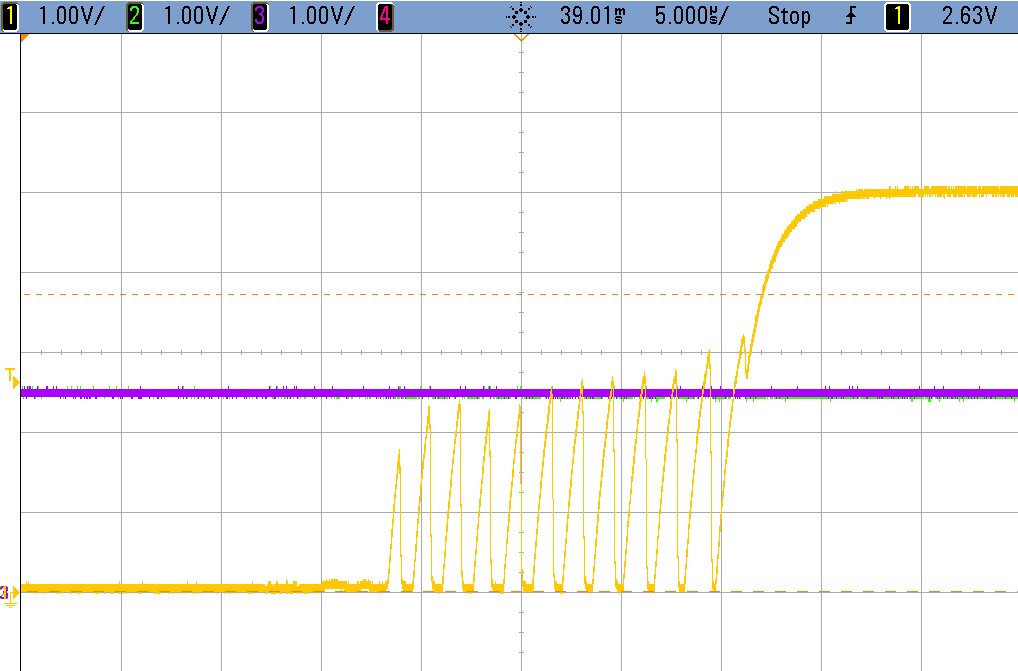
\includegraphics{figs/salida_comp.png}	
	}
	\caption{Salida del comparador (amarillo), cuando la tensi\'on del joystick (violeta) es superada por la señal triangular (verde).}
	\label{fig:salida_comp}
\end{figure}
%
\newpage
\section{Conclusi\'on}
%nombrar que solucionamos problemas y bla


\end{document}